\chapter{Particle Dynamics History (PDH)}\label{ch:pdh}
A particle carries its inertia, which is caused by changes in flow, such as vortices, shocks, expansion regions, sharp turns, and turbulence. These cause the particles that follow the flow to deviate from the flow path. Particle-based optical velocimetry experiments observe this particle field, capturing deviations in the velocity from the actual flow rather than the underlying flow features. This has traditionally been studied using the Stokes number of the particles, which is the ratio of the response time of the particles to the characteristic time scale of the flow. Particles with low Stokes numbers trace the flow more closely and are more suitable for optical velocimetry experiments such as particle image velocimetry (PIV).\par

The inertia experienced by the particles is compounded as they pass through a series of regions that accelerate them. Particle dynamics history (PDH) refers to this compounding effect that a particle experiences as it passes through a complex flow field with a wide range of flow features. This becomes particularly prominent when the flow is studied using experiments such as Particle Image Velocimetry (PIV) or Laser Doppler Velocimetry (LDV), as these experiments directly observe the particle field. The assumption in non-intrusive velocity measurement experiments is that the particle tracer velocity is the same as the flow surrounding it. This is untrue as a particle passes through a shock, and analytical relations have been provided using a correction to the Stokes drag by Melling \cite{melling1997}. Since then, this form of analysis has become popular for quantifying uncertainty related to the presence of tracer particles in particle-based velocimetry experiments. Samimy et al. \cite{samimy1991} recommended a Stokes number of less than 0.05 based on their numerical study of particles in a compressible free shear layer. This analysis considered the effect of particle dynamics downstream of the flow, which is indirectly attributed to the effect of PDH. In practice, the recommended Stokes number is unattainable for supersonic applications due to the effect of particle agglomeration, which is directly dependent on local flow properties. This has been observed in several works, such as Urban and Mungal \cite{urban2001} and Williams et al. \cite{williams2015}. Therefore, the study of PDH becomes important when studying flows using optical velocimetry.\par

\begin{figure}[ht!]
    \centering
    \centering
    \includesvg[width=0.8\linewidth]{./figures/02p5pdh/pdh_vortex}
    \caption{Demonstration of particle dynamics history (PDH) by spawning a particle at two different locations in an outgoing vortex field}
    \label{fig:PDH_demonstration}
\end{figure}

To better understand PDH, a hypothetical vortex field is used based on Murman et al. \cite{murman1989}. This is an outgoing velocity field with zero velocity in the center of the vortex. This field is chosen to demonstrate the concept of PDH, as the velocity at each point is different, resulting in a continuous drag force acting on the particle at any given point in the field, except at the spawn location. The particles are spawned at the flow velocity, which aligns with the particle-based velocimetry assumption of matching local flow velocity. The results obtained by passing particles with mass at different locations along the same streamline are shown in Fig. \ref{fig:PDH_demonstration}. This indicates that the particle spawned closer to the center of the vortex deviates farther from the streamline than the particle spawned midway. This suggests that the inertia experienced by the particle passing through an accelerating field is compounded by the drag force experienced over time. This particular effect, termed PDH, is undesirable in optical velocimetries. In most of these experiments, particles are spawned upstream to reach the local stream velocity before entering the interrogation area (IA). If this IA is large enough or has a field that evolves with implications for force on the particles, the PDH must be considered to get accurate data.\par

\section{Previous efforts to study PDH}
Several efforts have been made to understand the presence of particles in complex flow fields. However, the impact of the particle dynamics history was not evident at the time. These efforts were detailed in Kalagotla et al. \cite{kalagotla2018} and \cite{kalagotla2020} to provide more context to the PDH. In this section, the data from these works are summarized.\par

\subsection{Shock boundary layer interaction (SBLI) data}
One of the first steps in understanding PDH is to look at the path of particles through an SBLI. This work utilized PIV data from the University of Michigan wind tunnel test, which studied the physics of SBLI. The experimental campaigns were detailed in the work of Lapsa et al. \cite{lapsa2010} and Eagle et al. \cite{eagle2014}. CFD support was provided by a team at the University of Cincinnati, and their work is detailed in Galbraith \cite{galbraith2011} and Friedlander et al. \cite{friedlander2015}.  Data from these works are summarized in Fig. \ref{fig:1-5}. Lagrangian phase particulate data were obtained by spawning and tracking the particles in the CFD data using an internal code called Modified-VISUAL3 (MV3). The streamline plotting algorithm in the code was modified to track particles with mass. More details of the code were presented in Kalagotla \cite{kalagotlathesis2018}.\par

A result of interest that highlights the effect of PDH is shown in Fig. \ref{fig:particle_paths_sbli}.
The figure highlights the particle paths (red) and streamlines (blue) originating from the spawn location of these respective particles. From a qualitative perspective, it is evident that the particles deviate from the streamlines as the flow evolves. The camera sensors in PIV observe this particle field. The data obtained from this particle field are reported to the experimenter.\par

Furthermore, Kalagotla et al. \cite{kalagotla2018} provide a detailed methodology using the particle tracking code, along with its validation. A monodisperse particle assumption was used to generate these particle paths with a particle size of 281 nm and a density of 813 $\text{kg/m}^3$ as provided by the manufacturer. This work did not consider the effects of particle coalescence and breakup, which would present a significant deviation from the results presented and are studied in this work.\par

\begin{figure}
    \centering
    \includegraphics[width=0.5\linewidth]{./figures/02p5pdh/particle_paths_sbli.png}
    \caption{Traced particle paths (red) and respective streamlines (blue) through an SBLI highlighting the effect of PDH}
    \label{fig:particle_paths_sbli}
\end{figure}

A detailed quantitative analysis has shown that the particulate data performed better than almost twenty CFD simulations, highlighting the impact of particle presence in CFD. This can be better understood by quantifying the uncertainty in terms of PDH. This approach of locally quantifying the effect of particle presence is explored in further chapters using a test case.\par

\subsection{Rotor 37 flow field - Turbomachinery flow}
A detailed account of particle tracking analysis through a rotating flow field is presented here. Several studies to date have focused on the presence of tracers in nonintrusive methods for stationary transonic flows. However, these techniques have not been used to determine the velocity in rotating flows. Laser Freckle Anemometry (LFA) of NASA Rotor 37, conducted by Suder et al. \cite{suder1994}, is a prime example. Denton \cite{denton1997} compared multiple CFD results of the Rotor 37 with experimental data and concluded that the underprediction of relative Mach number after shock by the majority of numerical codes is due to their inability to correctly estimate the thickness of the boundary layer. The current work demonstrates that this overprediction of velocity by the experiment is partly or completely due to the inertia of the particle. The same post-processing code used for the previous case was used with a new methodology to track particles in a rotating field.\par

\section{Rotor 37 CFD data}\label{cfddata}
The CFD of Rotor 37 was thoroughly discussed using various codes in the work of Suder et al. \cite{suder1994}, Denton et al. \cite{denton1997}, and recently by Boretti et al. \cite{boretti2010}. For the current work, the CFD of Rotor 37 was performed using the well-established turbomachinery-specific code NUMECA \cite{fine2019} test case. The grid was generated using the built-in Autogrid5. Fine Turbo was used as the flow solver, and a Navier-Stokes model (RANS) coupled with the Spalart-Allmaras turbulence model was used to solve the flow. Compressible, perfect air was assumed as the flow medium. The boundary conditions used are the same as those of Suder et al. \cite{suder1994} computational analysis. A 0.356 mm tip clearance (0.014 in) or 0.6\% of the rotor tip chord was used. Analysis was conducted at the design speed for the specified design operating conditions. The initial estimated static pressure was set to 0.9MPa.\par

The grid for Rotor 37 in the current study consists of a structured nine-block grid. A grid resolution study was conducted using four different grid sizes, classified as coarse (843,093 nodes), medium (1,464,289 nodes), fine (2,079,637 nodes), and finer (2,922,481 nodes). None of the grids showed significant deviation in skewness angle, expansion ratio, and aspect ratio. It was also observed that there are no negative cells. Since this work aimed to compare the numerical data with the LFA results, the relative Mach number was considered for the resolution study. The relative Mach vs. \% chord obtained in a streamline with a span of 50\% of the blade and a pitch of 20\% is presented in Fig. \ref{relmachvschord}. The figure shows that the fine and finer grids do not exhibit significant deviations from each other, and the weighted average of the relative Mach number was found to be 0.07\%. Hence, the fine grid was chosen for all further analysis unless otherwise specified. Finally, an unformatted plot3D file was generated with the variables required from the stationary frame of reference to further process the results using MV3.\par

\begin{figure}[h!]
 \centering
 \includegraphics[width=0.7\linewidth]{./figures/02p5pdh/Grid_comparison}
 \caption{Grid resolution study depicting almost the same data with fine and finer grids}
 \label{relmachvschord}
\end{figure}

\subsubsection{Rotor 37 experimental data}\label{expdata}
Rotor 37 LFA data were obtained by Suder \cite{suder1996}. Particle lag is associated with the particle response time, which is the ability of a particle to react to changes in the flow field. It depends on the density ratio, particle size, and shape. In the experiment, polystyrene latex spheres (1050 $\text{kg/m}^3$) were used as tracers in the flow field. The range of particles used for the experiment was specified as 0.7 - 0.9 $\mu\text{m}$, and particles below 0.6 $\mu\text{m}$ were difficult to study due to low diffraction. The uncertainty in diameter in each batch of particles was uniform to within 0.1 $\mu\text{m}$. Therefore, the particle sizes were almost constant in each batch, but the mean particle size ranged between 0.7 and 0.9 $\mu\text{m}$. The particle sizes reported were obtained from scanning electron microscope (SEM) photographs. This does not account for the effect of particle agglomeration, which is significant, as noted in the works of Urban et al. \cite{urban2001} and Williams et al. \cite{williams2015}. Particle response analysis is necessary to accurately report the particle sizes to be used in numerical analysis. Due to this, the experimenter reported that the estimate of 5-8\% chord length uncertainty related to the presence of the particle would be on the lower estimate, and further analysis was needed for the particle size and density. This work examines the sizes reported by the experimenter to identify regions of high uncertainty through numerical particle tracing analysis. \par

In a flow field, the spatial resolution, or the spacing between data points, is an important factor in estimating the properties of the flow, particularly when there are high local accelerations. The Rotor 37 features an incoming bow shock and SBLI mechanism, as well as a passage shock, which makes data point spacing a crucial factor to consider when comparing experimental data with its respective CFD data. Data were reported to be collected at various spanwise and streamwise locations shown in Fig. \ref{fig:explocations}. In the spanwise direction, the resolution was set to a minimum of 2\% span near the tip and a maximum of 5\% span. LFA data was not obtained below 20\% span and above 98\% span. In the streamwise direction, the spacing of the data points was 5\% of the length of the rotor chord (approximately 3.0mm at the tip), and the data collected generally started one chord upstream of the rotor, went through the rotor, and ended one chord downstream of the rotor. In the pitchwise direction, the spacing is set at 184 points from blade to blade.\par

\begin{figure}[h!]
 \centering
 \includegraphics[width=0.7\linewidth]{./figures/02p5pdh/Survey_locations}
 \caption{Schematic of survey locations in the experimental investigation of Rotor 37; Credit: Suder \cite{suder1996}}
 \label{fig:explocations}
\end{figure}


\subsubsection{Analysis of Rotor 37 using MV3}\label{r37analysis}
MV3 has the ability to import multi-block structured plot3d data, which is the format exported by Numeca Fine. The initial import of Rotor 37 into MV3 is shown in Fig. \ref{fig:r37mv3}. The density is used as a scalar variable for the current visualization. The 2D plane shown in the figure is at a 70\% span. A particle can be spawned at any location by entering coordinates into the command window. This section presents the method for spawning particles in the current flow field and a test case to show that the particle lag in the Rotor 37 flow is considerable. In the current version of the MV3 code, only the drag force on the particle is tracked. Note that the centrifugal force acting on the particle in the relative frame is not considered, which might affect the current analysis. This force is planned to be added in future iterations of the code.\par

\begin{figure}[h!]
 \centering
 \includegraphics[width=0.7\linewidth]{./figures/02p5pdh/Initial_import}
 \caption{Initial import of the Rotor 37 into the MV3 code}
 \label{fig:r37mv3}
\end{figure}

\subsubsection{Method to spawn particles in rotating flow fields}
In any non-intrusive velocity measurement imaging techniques, the particles should reach the flow velocity before reaching the plane under observation. This is achieved in experiments by introducing particles far upstream of the area of interest. Similarly, this behavior can be mimicked in numerical analysis by spawning the particles upstream of the flow. However, the limitation for rotating machinery comes with the periodic condition that most codes use to reduce computational load.\par

\begin{figure}[h!]
 \centering
 \begin{subfigure}{.5\textwidth}
 \centering
 \includegraphics[width=\linewidth]{./figures/02p5pdh/3D_streamline_traces_2}
 \caption{3D view of 70\% span plane}
 \label{fig:upstreamlocation}
 \end{subfigure}%
 \begin{subfigure}{.5\textwidth}
 \centering
 \includegraphics[width=0.49\linewidth]{./figures/02p5pdh/Particle_spawn_location}
 \caption{The area of spawn and the plane under observation}
 \label{fig:spawnlocation}
\end{subfigure}
\caption{Particle spawn region and the observation plane}
\label{fig:particlespawn}
\end{figure}

For the current analysis, the region under observation is at 70\% span location between two successive blade rows. To study the particle characteristics in comparison to the flow, the particles must be spawned at an upstream location to allow them to pass through this region. This was achieved by tracing the streamlines back to an upstream location, as shown in Fig. \ref{fig:upstreamlocation}. It can be observed from the figure that the flow is highly three-dimensional, and the streamlines at any given point pass in and out of the plane. All streamlines passing through the area of interest originate from blade rows two and three; this is evident from Fig. \ref{fig:upstreamlocation}. If the radial velocity is considerable, this is a highly undesirable property for non-intrusive techniques like PIV. It should be noted that the streamlines in the separation region close to the trailing edge of the blade surface originate from far away; as such, the flow in this area is not captured for the current analysis. To populate the area of interest with particles, a total of seven blade rows were used. The particles are spawned with the local flow properties on an axial plane in the rectangular regions highlighted, as shown in Fig. \ref{fig:spawnlocation}. The plane under observation is also highlighted in the figure. The spacing between the particles is set to $7 \mu m$ in the radial direction and $10 \mu m$ in the transverse direction.\par

The particles are spawned in the axial plane using the MV3 code. The Stokes drag is employed for the current analysis. A particle spawned at any location using the MV3 code will initialize with the local flow velocity and track the flow with a constant time step. The code uses an explicit $4^{th}$ order Runge-Kutta method to integrate for the position. The CFL number for the entire analysis is set to a maximum of 0.1. The application of the code is more detailed in Kalagotla \cite{kalagotlathesis2018}. \par

The particles are tracked using the Lagrangian method. The MV3 code outputs particle data into a text file. The file consists of the location, velocity, and acceleration of both the particle and the fluid at every iteration. Each file can be used to generate a particle path and its respective streamline. On the basis of the number of particles spawned, the files will be generated. To generate the contours, all of this data is interpolated onto a plane linearly. Since care is taken to make sure the region under observation is densely populated with particles, the error from the interpolation is almost zero. The interpolated data are then plotted on a structured grid and analyzed.\par

\paragraph{A numerical particle response analysis}
Before proceeding with the main analysis, a test case was examined to determine if it is worthwhile to investigate the particle effects in Rotor 37. Particle sizes of 0.7, 0.8, and 0.9 $\mu\text{m}$ were chosen for the current study, as they are the sizes specified in the experimental work carried out by Suder \cite{suder1996}. The mean particle size of 0.8 $\mu\text{m}$ particles passes through an oblique shock with properties similar to the bow shock under the operating conditions of Rotor 37. The shock normal velocity vs. particle settling distance in terms of percentage chord length is shown in Fig. \ref{fig:clvssnv}. From the figure, it can be seen that the maximum particle relaxation distance was about 4.32\% of the chord length, which implies a significant impact on velocity estimation in that region. The particle relaxation time was calculated to be 0.265 $\mu \text{s}$. An estimate of the flow time scale was calculated based on the thickness of the boundary layer in the 70\% span and the free stream velocity as 1.370 $\mu \text{s}$. This produces a Stokes number of 0.193, which is quite high for a given particle. According to Samimy et al. \cite{samimy1991}, the Stokes number of a particle should be less than 0.05 to accurately predict the flow characteristics. Therefore, the current analysis to understand the particle behavior in the Rotor 37 flow should produce a reasonable difference between the CFD and the numerical-PIV (NPIV) data.\par

\begin{figure}[!ht]
 \centering
 \includegraphics[width=0.7\linewidth]{./figures/02p5pdh/R37_shocktest_PC}
 \caption{Particle settling distance in terms of \% chord using a test case}
 \label{fig:clvssnv}
\end{figure}

\subsubsection{Results and discussion}\label{results}
In this section, the difference between the CFD data and NPIV data is compared at the 70\% span location. Different particle sizes were tested to investigate their impact on predicting flow characteristics in Rotor 37. \par

\paragraph{Relative velocity contours}
At standard operating conditions, the steepest gradient in the flow field of Rotor 37 occurs at the shock interface of the passage. To understand the behavior of particles across this shock, the region around the shock is densely populated with particles. These particle data are interpolated into the 70\% span plane, as explained in Section \ref{r37analysis}. The results obtained, in contrast to the CFD data, are presented in Fig. \ref{fig:contour}. In the current analysis, the boundary condition at the surface is not set to no-slip; instead, particles hitting the domain boundary disappear, which can lead to erroneous results on the blade. Also, recall that the vortex structures in the separation zones are not captured. Hence, the data at the trailing edge is lost. All the results in this work have been corrected to avoid these regions. The other flow features should be accurate and maintain the behavior of the particles.\par

\begin{figure}[h!]
 \centering
 \includegraphics[width=0.7\linewidth]{./figures/02p5pdh/Contour}
 \caption{Relative velocity contours of NPIV and CFD highlighting the zones of interest}
 \label{fig:contour}
\end{figure}

In Fig. \ref{fig:contour}, the blades are numbered 1 \& 2. All features of the flow, including the bow shock, the reflected shock, and the accelerating region between the blades, are accurately captured in the NPIV data. The main difference between NPIV and CFD can be observed close to the pressure surface of the blade-2 after 50\% chord length. This region is also highlighted in the figure. Since this represents a significant deviation from the actual result, the concentration of the particles was increased in this region to minimize interpolation errors, if any. The high velocity in this region could be due to the interaction of the shock boundary layer of the rotor passage shock. Particles with inertia did not settle to post-shock velocity and were traversed through an expansion fan originating from the SBLI effect. Recall that the structure is three-dimensional and that the particles are moving in and out of the plane while traversing the SBLI structure. This could have caused the particles to accelerate in the highlighted region. This could be one of the reasons why the boundary layer thickness predicted by the CFD with tracers is higher than that observed in the experiments. Denton et al. in their work \emph{ ``Lessons from Rotor 37"}, stated that the higher thickness of the boundary layer in the CFD compared to the experiment is the reason for the overprediction of the pressure ratio. Figure \ref{fig:aaplot} shows the axial velocity plot along the line AA. The behavior of the particles discussed above close to the trailing edge of Blade 2 can be clearly understood from the plot. Along the BB line, whose plot is shown in Fig. \ref{fig:bbplot}, the NPIV data seemed to track flow features closely compared to the line AA. This could be due to the longer settling times for the particle to reach post-shock velocity before passing through the accelerating region.\par

The other deviation in the flow features between NPIV and CFD was observed in the shape of the rotor passage shock. The shock structure generated from the particle data looked smeared compared to the CFD structure. The reason for this behavior can be attributed to the fact that the particles passing through the shock have varying velocities at different pitch locations.\par

\begin{figure}[hbt!]
\centering
\begin{subfigure}{.5\textwidth}
\centering
\includegraphics[width=\linewidth]{./figures/02p5pdh/AA}
\caption{Along AA}
\label{fig:aaplot}
\end{subfigure}%
\begin{subfigure}{.5\textwidth}
\centering
\includegraphics[width=0.97\linewidth]{./figures/02p5pdh/BB}
\caption{Along BB}
\label{fig:bbplot}
\end{subfigure}
\caption{Relative velocity of NPIV vs. CFD data}
\label{fig:RVline}
\end{figure}


\paragraph{Evaluation of the particle response}
This analysis was conducted to understand how the particle size or Stokes number affects the flow characteristics of Rotor 37. The particles passing through 70\% span close to the pressure surface of the blade due to the deviation from the path discussed in the previous section. The particle lag is expected to be significant across two regions in the flow field, the bow shock and the passage shock. The data obtained from these regions are analyzed and presented in Fig. \ref{fig:particleresponse}. Figures show the relative velocity of the particle compared to the flow velocity at different axial locations. From the figures, it can be seen that the particle deviation behind the bow shock is considerable compared to the passage shock. Although the passage shock has the steepest gradient inside the rotor blades, the normal bow shock is where the particle lag seems to be the maximum, and is also the region of high error in this case. The result obtained agrees with the fact that the Stokes number is the major factor affecting the prediction of flow behavior by experiments. Careful observation of Fig. \ref{fig:leftzoom} shows that the particle with a high Stokes number never reached the flow velocity after passing through the bow shock. This implies that a high-velocity region can be expected in the NPIV data compared to the CFD in this region, as discussed above.\par

\begin{figure}[hbt!]
\centering
\begin{subfigure}{.5\textwidth}
\centering
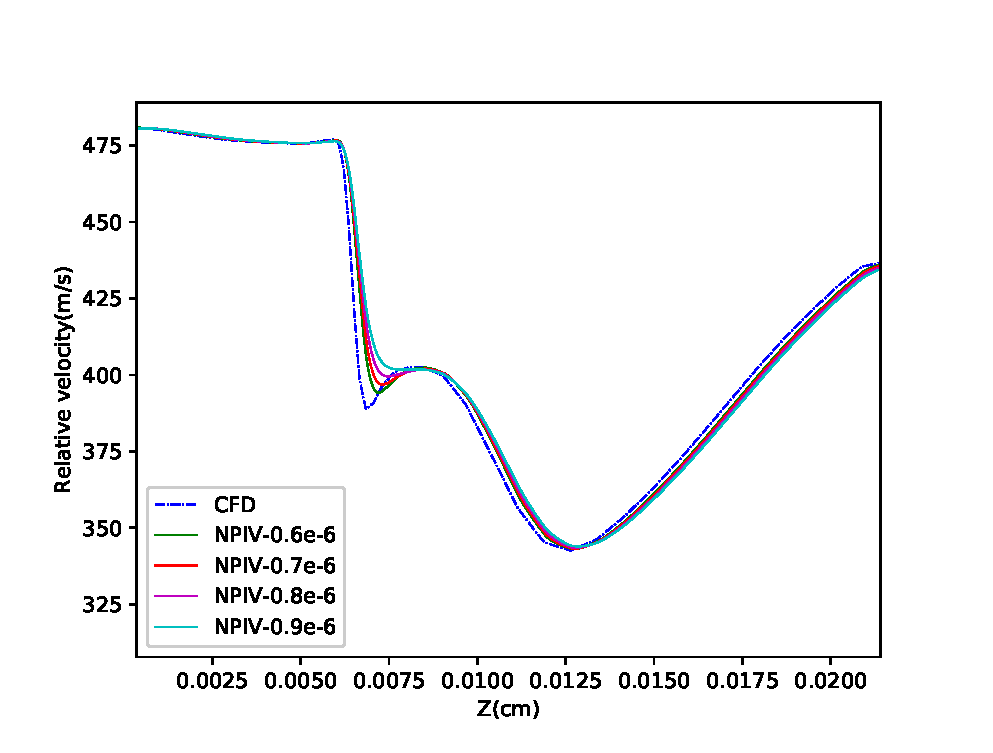
\includegraphics[width=\linewidth]{./figures/02p5pdh/Left_zoom}
\caption{Bow shock to Passage shock}
\label{fig:leftzoom}
\end{subfigure}%
\begin{subfigure}{.5\textwidth}
\centering
\includegraphics[width=\linewidth]{./figures/02p5pdh/Right_zoom}
\caption{Passage shock to Trailing edge}
\label{fig:rightzoom}
\end{subfigure}
\caption{Relative velocity profiles close to the pressure surface}
\label{fig:particleresponse}
\end{figure}

\section{Framework to study the PDH}
It is important to consider particle lag when validating steady-state numerical data in non-intrusive particle-based experiments. Multiple works, such as Lazar et al. \cite{lazar2010}, Burns et al. \cite{burns2015}, Kalagotla et al. \cite{kalagotla2018}, and Kalagotla et al. \cite{kalagotla2020}, have shown that considering particle dynamics improves the validation accuracy between the data. However, these studies have been case-specific. The current methodology aims to generalize and extend to all numerical code validations.\par

\begin{figure}[ht!]
	\centering
	\includesvg[scale=1.2]{./figures/02p5pdh/PDH_syPIV_workflow}
	\caption{Methodology to generate PDH informed numerical data (black path) and traditional way of generating synthetic images (red path)}
	\label{fig:workflows}
\end{figure}

The methodology to inform the CFD data with PDH is shown in Fig. \ref{fig:workflows}. The steady-state data can be processed by spawning particles upstream of the flow. These particles are tracked in the Lagrangian frame using one-way coupling. This captures the effect of PDH as these particles navigate through the flow. This closely replicates the presence of tracer particles in optical velocimetry experiments, such as PIV. The obtained particle data can be transformed to the Eulerian frame using grid interpolation techniques for further processing. These data have information from PDH and are more suitable for validation with the experimental data. Synthetic images generated from these data can quantify the uncertainty related to the presence of particles, the imaging phase, and the image processing phase of PIV. This method can be extended to any velocimetry using tracers. The tools used for the framework presented in Fig. \ref{fig:workflows} are detailed in further chapters.\par


\section{Summary}
The work presented here highlights that the particle dynamics history (PDH) plays a significant role in the measurements obtained from optical velocimetries. Although the theory of PDH was not presented at the time of publication of the work, the results demonstrated the impact of PDH-informed data in contrast to CFD or optical velocimetry data. The results obtained from these analyses are difficult to interpret due to the presence of complex interactions. To solidify the proposed theory of PDH, a methodology is established to quantify its effect using several tools. These tools are explored in the following chapters.\par